% !TeX program = xelatex
\documentclass[a4paper,10pt]{article}

% ============================================================================
% សន្លឹកកិច្ចការសិស្ស ស-ខ្មៅ (Student Worksheet - Grade 8 Lesson 1: 6 RAT_PROB)
% បរិបទ៖ គ្មានស្លាយ LCD និងគ្មានម៉ាស៊ីនគិតលេខ — សិស្សបំពេញផ្ទាល់លើសន្លឹកកិច្ចការ ២ ទំព័រ A4
% ============================================================================
\usepackage[a4paper, left=0.85cm, right=0.85cm, top=0.70cm, bottom=0.95cm, footskip=0.48cm]{geometry}
\usepackage{amsmath, amssymb}
\usepackage{unicode-math}
\usepackage{fontspec}
\usepackage{array, colortbl}
\usepackage[table]{xcolor}
\usepackage{enumitem}
\usepackage{pifont}
\usepackage{fancyhdr}
\usepackage{lastpage}
\usepackage{tikz}
\usepackage[most]{tcolorbox}
\usetikzlibrary{calc, arrows.meta, decorations.pathreplacing, positioning, babel}

\makeatletter
\let\@expl@@@mark@update@singlecol@structures@@\relax
\makeatother

\providecommand{\NGSFindFonts}{%
  \IfFileExists{C:/Windows/Fonts/cambria.ttc}{%
    \def\NGSSysPath{C:/Windows/Fonts/}%
    \def\NGSUserPath{C:/Users/KIT/AppData/Local/Microsoft/Windows/Fonts/}%
  }{%
    \IfFileExists{./fonts/KhmerOSsiemreap.ttf}{\def\NGSSysPath{./fonts/}\def\NGSUserPath{./fonts/}}{%
    \IfFileExists{../fonts/KhmerOSsiemreap.ttf}{\def\NGSSysPath{../fonts/}\def\NGSUserPath{../fonts/}}{%
    \IfFileExists{../../fonts/KhmerOSsiemreap.ttf}{\def\NGSSysPath{../../fonts/}\def\NGSUserPath{../../fonts/}}{%
    \IfFileExists{../../../fonts/KhmerOSsiemreap.ttf}{\def\NGSSysPath{../../../fonts/}\def\NGSUserPath{../../../fonts/}}{%
    \IfFileExists{../../../../fonts/KhmerOSsiemreap.ttf}{\def\NGSSysPath{../../../../fonts/}\def\NGSUserPath{../../../../fonts/}}{%
    \IfFileExists{../../../../../fonts/KhmerOSsiemreap.ttf}{\def\NGSSysPath{../../../../../fonts/}\def\NGSUserPath{../../../../../fonts/}}{%
    \IfFileExists{../../../../../../fonts/KhmerOSsiemreap.ttf}{\def\NGSSysPath{../../../../../../fonts/}\def\NGSUserPath{../../../../../../fonts/}}{%
      \def\NGSSysPath{../../../../../../../fonts/}\def\NGSUserPath{../../../../../../../fonts/}%
    }}}}}}}%
  }%
}
\NGSFindFonts

\setmathfont[Path={\NGSSysPath}, FontIndex=1, Scale=1.02]{cambria.ttc}
\defaultfontfeatures{Ligatures=TeX}

\setmainfont[
  Path={\NGSUserPath}, Extension=.ttf, Script=Khmer,
  BoldFont={KhmerOSsiemreap}, BoldFeatures={FakeBold=1.8},
  ItalicFont={KhmerOSsiemreap}, ItalicFeatures={FakeSlant=0.22}
]{KhmerOSsiemreap}

\newfontfamily\muol[Path={\NGSUserPath}, Extension=.ttf, Script=Khmer]{KhmerOSmuollight}
\newfontfamily\TimesEn[Path={\NGSSysPath}, Extension=.ttf, BoldFont={timesbd}, ItalicFont={timesi}]{times}

\XeTeXlinebreaklocale "km"
\XeTeXlinebreakskip = 0pt plus 1pt minus 0.1pt

\definecolor{panelgray}{gray}{0.93}
\definecolor{headgray}{gray}{0.85}

\pagestyle{fancy}
\fancyhf{}
\renewcommand{\headrulewidth}{0pt}
\fancyfoot[L]{\fontsize{7.5pt}{9.5pt}\selectfont អនុវិទ្យាល័យព្រះក្រសាំង \en{|} គណិតវិទ្យាថ្នាក់ទី៨ \en{|} មេរៀនទី១៖ ៦. ចំណោទ និងសំយោគមេរៀនទី១ (គ្រូ៖ ហុក ប៊ុនថែន)}
\fancyfoot[R]{\fontsize{7.8pt}{9.5pt}\selectfont ទំព័រ \en{\thepage/\pageref{LastPage}}}

\setlength{\parindent}{0pt}
\setlength{\parskip}{0pt}
\setlength{\tabcolsep}{3.8pt}

\newcommand{\en}[1]{{\TimesEn #1}}
\newcommand{\enbf}[1]{{\TimesEn\bfseries #1}}
\newcommand{\unit}[1]{\,\text{\en{#1}}}
\newcommand{\cnum}[1]{\mbox{\fontsize{10pt}{12pt}\selectfont\ding{\numexpr181+#1\relax}}}
\newcommand{\chkbox}{\tikz[baseline=-0.12ex]\draw[black, line width=0.8pt] (0,0) rectangle (0.24cm,0.24cm);}
\newcommand{\blank}[1][1.5cm]{\makebox[#1]{\dotfill}}
\newcommand{\secbar}[2]{%
  \begin{tcolorbox}[enhanced, sharp corners, colback=headgray, colframe=black, boxrule=0.9pt, boxsep=1pt, top=2pt, bottom=2pt, left=5pt, right=5pt, before skip=4pt, after skip=3pt]
    {\muol\fontsize{9.2pt}{13pt}\selectfont #1}\hfill{\fontsize{8pt}{11pt}\selectfont\textbf{#2}}
  \end{tcolorbox}%
}

\newcolumntype{L}[1]{>{\raggedright\arraybackslash}p{#1}}
\newcolumntype{C}[1]{>{\centering\arraybackslash}p{#1}}

\begin{document}
\fontsize{9.6pt}{14.4pt}\selectfont

% ============================================================================
% ទំព័រទី ១៖ E1 + E2 (POE 1 & POE 2) + E3 សំយោគបញ្ញត្តិ និងធនាគារហេតុផល
% ============================================================================
\begin{tcolorbox}[enhanced, sharp corners, colback=white, colframe=black, boxrule=1.0pt, boxsep=2pt, top=3pt, bottom=3pt, left=6pt, right=6pt]
  \begin{center}
    {\muol\fontsize{9.8pt}{14.8pt}\selectfont អនុវិទ្យាល័យព្រះក្រសាំង \enbf{--} សន្លឹកកិច្ចការសិស្ស \enbf{(}មេរៀនទី១៖ ៦\enbf{.} ចំណោទ និងសំយោគមេរៀនទី១\enbf{)}}\\[3pt]
    {\fontsize{8.8pt}{12pt}\selectfont
    ឈ្មោះសិស្ស / ដៃគូ៖ \blank[5.2cm] \hspace{0.25cm}
    ថ្នាក់ទី៨៖ \blank[1.1cm] \hspace{0.25cm}
    ក្រុមទី៖ \blank[1.0cm] \hspace{0.25cm}
    កាលបរិច្ឆេទ៖ ២៣/១១/២០២៦}
  \end{center}
\end{tcolorbox}

% --- E1 + E2 ---
\secbar{ផ្នែកទី១៖ បេសកកម្មគូប្រភាគអច្ឆរិយៈ \enbf{(E1)} និងការរុករកចំណោទជាដៃគូ \enbf{(E2 -- POE 1 \& POE 2)}}{រយៈពេល ១៤ នាទី}

\begin{tcolorbox}[enhanced, sharp corners, colback=panelgray, colframe=black, boxrule=0.75pt, boxsep=1.5pt, top=2.5pt, bottom=2.5pt, left=5pt, right=5pt]
  \textbf{បេសកកម្ម \en{E1} (លំហាត់ \#11 ទំ.១២ — ទស្សន៍ទាយមុនគណនា)៖} តើ $\frac{13}{4}+\frac{13}{9}$ ស្មើនឹង $\frac{13}{4}\times\frac{13}{9}$ មែនឬទេ? \chkbox\ ពិត \quad \chkbox\ មិនពិត\\[3pt]
  $\bullet$ គណនាផ្ទៀងផ្ទាត់៖ (១) $\dfrac{13}{4}+\dfrac{13}{9} = \dfrac{\blank[0.9cm] + 52}{36} = \blank[1.2cm]$ \quad \en{|} \quad (២) $\dfrac{13}{4}\times\dfrac{13}{9} = \blank[1.2cm]$ \quad (ព្រោះ $4+9=\blank[0.7cm]$!)
\end{tcolorbox}

\vspace{4.5pt}
\textbf{ក. សកម្មភាពទី ១ (\en{POE 1})៖ គំនូសប្លង់ចតុកោណកែង ៤ ជំហាន (ចំណោទសៀវភៅពុម្ព ទំ.១០–១១)}

\begin{tcolorbox}[enhanced, sharp corners, colback=white, colframe=black, boxrule=0.7pt, boxsep=2pt, top=3pt, bottom=3pt, left=5pt, right=5pt]
  \begin{minipage}{13.1cm}
    ចតុកោណកែងមួយមានបរិមាត្រ $P = 16.38\unit{cm}$ និងជ្រុងមួយស្មើនឹង $3.26\unit{cm}$ ៖\\[3.5pt]
    $\bullet$ \textbf{ក) រកកន្លះបរិមាត្រ $p$៖} $p = 16.38 \div 2 = \blank[1.5cm]\unit{cm}$ (\textbf{ប្រយ័ត្ន៖} កុំយក $16.38-3.26$ ភ្លាម!)\\[3.5pt]
    $\bullet$ \textbf{ខ) តាង $x$ ជាជ្រុងមួយទៀត៖} $x + 3.26 = \blank[1.1cm] \implies x = \blank[1.1cm] - 3.26 = \blank[1.2cm]\unit{cm}$\\[3.5pt]
    $\bullet$ \textbf{គ) គណនាផ្ទៃក្រឡា $S$៖} $S = 3.26 \times \blank[1.2cm] = \blank[1.8cm]\unit{cm}^2$\\[3.5pt]
    $\bullet$ \textbf{ឃ) ផ្ទៀងផ្ទាត់បរិមាត្រ៖} $P = 2\times(x + 3.26) = 2\times\blank[1.2cm] = \blank[1.4cm]\unit{cm}$ (\cnum{5})
  \end{minipage}\hfill
  \begin{minipage}{4.4cm}
    \centering
    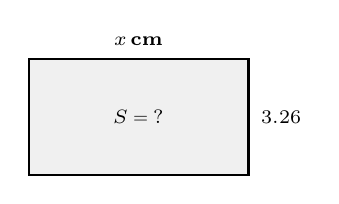
\begin{tikzpicture}[x=0.90cm, y=0.84cm, every node/.style={font=\scriptsize, text=black}]
      \draw[black, line width=0.9pt, fill=gray!12] (0,0) rectangle (3.1,1.75);
      \node at (1.55,2.02) {\textbf{$x\unit{cm}$}};
      \node at (1.55,0.88) {$S = ?$};
      \node[anchor=west] at (3.15,0.88) {$3.26$};
    \end{tikzpicture}
  \end{minipage}
\end{tcolorbox}

\vspace{5pt}
\textbf{ខ. សកម្មភាពទី ២ (\en{POE 2})៖ ដ្យាក្រាមផ្លិតបំណែងចែកប្រាក់ប្រចាំខែ (លំហាត់ \#14 ទំ.១២)}

\begin{tcolorbox}[enhanced, sharp corners, colback=white, colframe=black, boxrule=0.7pt, boxsep=2pt, top=3pt, bottom=3pt, left=5pt, right=5pt]
  \begin{minipage}{13.3cm}
    គ្រួសារមួយបែងចែកប្រាក់ប្រចាំខែលើ៖ ម្ហូប $\frac{1}{2}$, ធ្វើដំណើរ $\frac{1}{20}$, កំសាន្ត $\frac{1}{10}$, ទឹក-ភ្លើង $\frac{1}{25}$ និងប្រាក់សន្សំ ($\text{\en{PPCM}} = 100$)៖\\[4pt]
    (១) ផលបូកចំណាយទាំង ៤៖ $\dfrac{1}{2}+\dfrac{1}{20}+\dfrac{1}{10}+\dfrac{1}{25} = \dfrac{50 + \blank[0.6cm] + \blank[0.6cm] + \blank[0.6cm]}{100} = \dfrac{\blank[0.8cm]}{100}$\\[4pt]
    (២) ប្រភាគប្រាក់សន្សំ (ដកពីឯកតាពេញ $1$)៖ $1 - \dfrac{\blank[0.8cm]}{100} = \dfrac{100 - \blank[0.8cm]}{100} = \blank[1.3cm]$
  \end{minipage}\hfill
  \begin{minipage}{4.2cm}
    \centering
    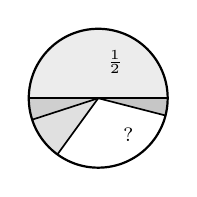
\begin{tikzpicture}[scale=0.84, every node/.style={font=\scriptsize, text=black}]
      \fill[gray!15] (0,0) -- (0:1.05) arc (0:180:1.05) -- cycle;
      \fill[gray!38] (0,0) -- (180:1.05) arc (180:198:1.05) -- cycle;
      \fill[gray!24] (0,0) -- (198:1.05) arc (198:234:1.05) -- cycle;
      \fill[gray!45] (0,0) -- (345.6:1.05) arc (345.6:360:1.05) -- cycle;
      \draw[black, line width=0.8pt] (0,0) circle (1.05);
      \foreach \ang in {0,180,198,234,345.6} { \draw[black, line width=0.6pt] (0,0) -- (\ang:1.05); }
      \node at (90:0.55) {ម្ហូប $\frac{1}{2}$};
      \node at (290:0.58) {\textbf{សន្សំ $?$}};
    \end{tikzpicture}
  \end{minipage}
\end{tcolorbox}

% --- E3 ---
\secbar{ផ្នែកទី២៖ សំយោគវិធីដោះស្រាយចំណោទ \enbf{(E3)} និងធនាគារហេតុផល \enbf{B\&W} \cnum{1}\enbf{--}\cnum{5}}{សៀវភៅពុម្ព ទំ.១០–១២}

\begin{tabular}{|L{9.20cm}|L{9.20cm}|}
  \hline
  \textbf{១. ជំហានទាំង ៤ ក្នុងការដោះស្រាយចំណោទចំនួនសនិទាន៖}\par\vspace{3pt}
  $\bullet$ \textbf{ជំហានទី១៖} គូស \blank[1.8cm] និងតាងអញ្ញាត (ឧ. $p, x, S$)\par\vspace{3pt}
  $\bullet$ \textbf{ជំហានទី២៖} សរសេរ \blank[2.0cm] គណិតវិទ្យាពីបម្រាប់\par\vspace{3pt}
  $\bullet$ \textbf{ជំហានទី៣៖} គណនាដោយដៃតាមលំដាប់អាទិភាពប្រមាណវិធី\par\vspace{3pt}
  $\bullet$ \textbf{ជំហានទី៤៖} ផ្ទៀងផ្ទាត់ភាពសមហេតុផល និងដាក់ \blank[1.5cm] ត្រឹមត្រូវ
  &
  \textbf{២. ធនាគារហេតុផល \en{B\&W} (\cnum{1}--\cnum{5})៖}\par\vspace{3pt}
  \cnum{1} ចតុកោណកែង៖ កន្លះបរិមាត្រ $p = P\div 2 = a+b$ និង $S = a\cdot b$ ។\par\vspace{3pt}
  \cnum{2} ដ្យាក្រាមផ្លិត/ឯកតាពេញ $1$៖ ផ្នែកនៅសល់ $= 1 - (\text{ផលបូកផ្នែកស្គាល់})$ ។\par\vspace{3pt}
  \cnum{3} ប្រភាគធំ $\frac{A}{B}$៖ គណនា $A$ ដាច់ និង $B$ ដាច់សិន រួចប្ដូរជា $A\div B$ ។\par\vspace{3pt}
  \cnum{4} អាទិភាព៖ វង់ក្រចក $\to$ គុណ/ចែក $\to$ បូក/ដក (ឬទាញកត្តារួម) ។\par\vspace{3pt}
  \cnum{5} ផ្ទៀងផ្ទាត់ខ្នាត៖ ប្រវែង ($\unit{cm}$), ក្រឡាផ្ទៃ ($\unit{cm}^2$), ផលបូកប្រភាគ $=1$ ។ \\
  \hline
\end{tabular}

\vspace{5pt}
\begin{tcolorbox}[enhanced, sharp corners, colback=panelgray, colframe=black, boxrule=0.75pt, boxsep=1.5pt, top=3pt, bottom=3pt, left=5pt, right=5pt]
  \textbf{ប្រយ័ត្នអន្ទាក់ដាច់ខាត៖} (១) ស្គាល់បរិមាត្រ $P$ ត្រូវចែកនឹង $2$ រកកន្លះបរិមាត្រ $p$ ជាមុនសិន (ហាមយក $P - a$ ភ្លាមៗ!) ។\\
  (២) ក្នុងកន្សោមចម្រុះ ត្រូវធ្វើវង់ក្រចក និងគុណ/ចែកមុនបូក/ដកជានិច្ច (\cnum{4}) និងកុំភ្លេចដាក់ខ្នាត $\unit{cm}$ ឬ $\unit{cm}^2$ (\cnum{5})!
\end{tcolorbox}

\vspace{5pt}
\textbf{៣. លំហាត់ត្រួតពិនិត្យរហ័ស៖ សំយោគប្រមាណវិធីទាំង ៤ និងខ្នាតរង្វាស់}

\vspace{3pt}
{\renewcommand{\arraystretch}{1.68}
\begin{tabular}{|C{4.40cm}|C{4.40cm}|C{4.40cm}|C{4.40cm}|}
  \hline
  \rowcolor{panelgray}
  \rule[-9pt]{0pt}{24pt}$P=10\unit{cm} \implies p=\blank[0.85cm]$ & $1 - \frac{7}{20} = \blank[1.05cm]$ & $\frac{1}{2}+\frac{1}{2}\times\frac{1}{3} = \blank[0.85cm]$ & $\frac{-5}{-1} = \blank[1.05cm]$ \\
  \hline
  \rule[-9pt]{0pt}{24pt}$p=8.5,\; a=3.2:\; b=\blank[0.70cm]$ & $\frac{3}{2^4} = \frac{3}{\blank[0.70cm]}$ & $\left(-\frac{2}{5}\right)\div\left(-\frac{4}{5}\right) = \blank[0.75cm]$ & $\frac{1}{2}\div\left(\frac{1}{4}+\frac{1}{4}\right) = \blank[0.70cm]$ \\
  \hline
  \rule[-9pt]{0pt}{24pt}$a=2.5,\; b=4 \implies S=\blank[0.70cm]$ & $1 - \left(\frac{1}{2}+\frac{1}{4}\right) = \blank[0.80cm]$ & $(-3)\times\left(-\frac{5}{6}\right) = \blank[0.85cm]$ & $0.25 + \frac{3}{4} = \blank[0.95cm]$ \\
  \hline
  \rule[-9pt]{0pt}{24pt}$(-2)\times(-2)\times(-2)=\blank[0.65cm]$ & $\frac{2}{3}\div\frac{4}{9} = \blank[0.90cm]$ & $-\frac{3}{8} + \frac{5}{8} = \blank[0.90cm]$ & $\left(-\frac{3}{5}\right)\times\left(-\frac{5}{3}\right) = \blank[0.70cm]$ \\
  \hline
\end{tabular}}

\newpage

% ============================================================================
% ទំព័រទី ២៖ E4 លំហាត់សំយោគ + E5 ចំណោទអនុវត្តន៍ & វិនិច្ឆ័យ A-D + Exit + កិច្ចការផ្ទះ
% ============================================================================
\secbar{ផ្នែកទី៣៖ ពង្រីកចំណេះដឹងលើប្រភាគធំ និងលក្ខណៈបំបែក \enbf{(E4 --} សៀវភៅពុម្ព ទំ\enbf{.}១២\enbf{)}}{រយៈពេល ១០ នាទី}

\textbf{លំហាត់សំយោគមេរៀនទី១៖} ចូរបំពេញជំហានគណនាខាងក្រោមដោយដៃ ព្រមទាំងបញ្ជាក់លេខហេតុផល \cnum{1}--\cnum{5}៖

{\renewcommand{\arraystretch}{1.58}
\begin{tabular}{|L{4.70cm}|L{9.10cm}|C{4.00cm}|}
  \hline
  \rowcolor{headgray}
  \textbf{លំហាត់សំយោគ (ទំ.១២)} & \textbf{ដំណើរការបំបែក និងគណនាដោយដៃតាមលំដាប់} & \textbf{ចម្លើយ និងហេតុផល} \\
  \hline
  \textbf{១. ប្រភាគធំ (ទំ.១២ \#9ច)}\par\vspace{3pt}$\left(3\dfrac{2}{5}-\dfrac{25}{8}\right) \Big/ \left(\dfrac{-7}{12}+5\dfrac{4}{9}\right)$ & \rule{0pt}{14pt}ភាគយក $A = \dfrac{136-125}{40} = \dfrac{\blank[0.65cm]}{40}$\par\vspace{3.5pt}ភាគបែង $B = \dfrac{-21+196}{36} = \dfrac{\blank[0.75cm]}{36}$\par\vspace{3.5pt}$\implies A\div B = \dfrac{11}{40}\times\dfrac{36}{175}$ (សម្រួលនឹង $4$)\rule[-8pt]{0pt}{8pt} & $=\blank[1.4cm]$ (\cnum{3}) \\
  \hline
  \textbf{២. វង់ក្រចកគុណប្រភាគ (\#10គ)}\par\vspace{2pt}$\left(-\dfrac{11}{13}+\dfrac{17}{16}\right)\cdot\dfrac{26}{22}$ & \rule{0pt}{16pt}គណនាក្នុងវង់ក្រចក៖ $=\left(\dfrac{-176+\blank[0.8cm]}{208}\right)\cdot\dfrac{13}{11} = \dfrac{45}{208}\cdot\dfrac{13}{11}$\rule[-8pt]{0pt}{8pt} & $=\blank[1.4cm]$ (\cnum{4}) \\
  \hline
  \textbf{៣. បង្ហាញលក្ខណៈបំបែក (\#12)}\par\vspace{2pt}$\dfrac{a}{b}\cdot\left(\dfrac{c}{d}-\dfrac{e}{f}\right)$ & \rule{0pt}{15pt}ប្ដូរដកជាបូកចំនួនផ្ទុយ៖ $=\dfrac{a}{b}\cdot\left[\dfrac{c}{d}+\left(\blank[1.0cm]\right)\right] = \dfrac{a}{b}\cdot\dfrac{c}{d} - \blank[1.2cm]$\rule[-8pt]{0pt}{8pt} & ពិត (\cnum{4}) \\
  \hline
\end{tabular}}

\vspace{4pt}
$\bullet$ \textbf{សំណួរឆ្លុះបញ្ចាំង \en{(EIA Looking-Back)}៖} ហេតុអ្វីក្នុងប្រភាគធំ \#9ច យើងគួរគណនាភាគយក $A$ និងភាគបែង $B$ ដាច់ពីគ្នាជាមុន?\\
ចម្លើយ៖ ដើម្បីចៀសវាងការភាន់ច្រឡំសញ្ញា រួចប្ដូររបារប្រភាគធំទៅជាសញ្ញា \blank[0.8cm] តាមក្បួន [រក្សាទុក-គុណ-ច្រាស] (\cnum{3})!

% --- E5 ---
\secbar{ផ្នែកទី៤៖ វាយតម្លៃលទ្ធផលសិក្សា \enbf{(E5 --} ចំណោទអនុវត្តន៍ \enbf{+} វិនិច្ឆ័យ \enbf{A--D +} សំបុត្រចេញ\enbf{)}}{រយៈពេល ១០ នាទី}

\textbf{ក. ចំណោទអនុវត្តន៍ និងអសមភាព (\#13 ទំ.១២ — ធ្វើជាដៃគូ រួចប្ដូរសន្លឹកផ្ទៀងផ្ទាត់ \en{Pause-Review})៖}

{\renewcommand{\arraystretch}{1.48}
\begin{tabular}{|L{10.00cm}|L{7.80cm}|}
  \hline
  \textbf{១) ចំណោទរងបន្លែសាលារៀន៖} រងបន្លែរាងចតុកោណកែងមួយមានបរិមាត្រ $P = 12.4\unit{m}$ និងទទឹង $2.5\unit{m}$ ។\par\vspace{2.5pt}
  $\bullet$ កន្លះបរិមាត្រ៖ $p = 12.4\div 2 = \blank[1.3cm]\unit{m}$ (\cnum{1})\par\vspace{2.5pt}
  $\bullet$ បណ្ដោយ៖ $x = \blank[1.1cm] - 2.5 = \blank[1.3cm]\unit{m}$\par\vspace{2.5pt}
  $\bullet$ ផ្ទៃក្រឡា៖ $S = 2.5 \times \blank[1.1cm] = \blank[1.4cm]\unit{m}^2$ (\cnum{5})
  &
  \textbf{២) ផ្ទៀងផ្ទាត់អសមភាព (\#13 ទំ.១២) និងបិទ \en{E1}៖}\par\vspace{2.5pt}
  $\bullet$ គេមាន $\dfrac{1}{3} < \dfrac{1}{2}$ ។ បូក $\dfrac{1}{6}$ ទាំងសងខាង៖\par\vspace{2.5pt}
  $\dfrac{1}{3}+\dfrac{1}{6} = \blank[1.0cm]$ និង $\dfrac{1}{2}+\dfrac{1}{6} = \blank[1.0cm]$ (\chkbox\ ពិត)\par\vspace{2.5pt}
  $\bullet$ \textbf{បិទ \en{E1}៖} $\dfrac{13}{4}+\dfrac{13}{9} = \dfrac{13}{4}\times\dfrac{13}{9} = \blank[1.2cm]$ \\
  \hline
\end{tabular}}

\vspace{5pt}
\textbf{ខ. គូសវង់ជុំវិញជម្រើសត្រឹមត្រូវតែ ១ គត់ ក្នុងចំណោម \en{A, B, C, D} រួចសរសេរលេខហេតុផល \cnum{1}--\cnum{5}៖}

{\renewcommand{\arraystretch}{1.72}
\begin{tabular}{|L{8.90cm}|L{8.90cm}|}
  \hline
  \rule[-9pt]{0pt}{24pt}\textbf{ជម្រើស \en{A}៖} $P=16.38,\; a=3.26 \implies x = 16.38-3.26 = 13.12$ &
  \textbf{ជម្រើស \en{B}៖} ប្រាក់សន្សំ $= 1 - \dfrac{69}{100} = \dfrac{31}{100}$ \\
  \hline
  \rule[-9pt]{0pt}{24pt}\textbf{ជម្រើស \en{C}៖} $\dfrac{1}{2} + \dfrac{1}{3}\div\dfrac{5}{6} = \dfrac{5}{6}\div\dfrac{5}{6} = 1$ &
  \textbf{ជម្រើស \en{D}៖} ផ្ទៃក្រឡាចតុកោណកែងមានខ្នាតគិតជា $\unit{cm}$ \\
  \hline
\end{tabular}}

\vspace{5pt}
\begin{tcolorbox}[enhanced, sharp corners, colback=panelgray, colframe=black, boxrule=0.75pt, boxsep=1.5pt, top=2.5pt, bottom=2.5pt, left=5pt, right=5pt]
  \textbf{សំបុត្រចេញពីថ្នាក់ (\en{Exit Ticket} — ៦០ វិនាទី)៖} គណនាតាមលំដាប់អាទិភាពប្រមាណវិធី៖\\
  $\dfrac{3}{4} - \dfrac{1}{4}\div\dfrac{1}{2} = \dfrac{3}{4} - \left(\dfrac{1}{4}\times\blank[1.0cm]\right) = \dfrac{3}{4} - \blank[1.0cm] = \blank[1.2cm]$ \quad (ហេតុផល៖ \blank[1.1cm])
\end{tcolorbox}

% --- កិច្ចការផ្ទះ ---
\secbar{ផ្នែកទី៥៖ កិច្ចការផ្ទះសំយោគ និងបុរេសិក្សាភ្ជាប់មេរៀនទី២ \enbf{(}ស្វ័យគុណ\enbf{)}}{ធ្វើក្នុងសៀវភៅកិច្ចការផ្ទះ}
$\bullet$ \textbf{លំហាត់ ១ (ភ្ជាប់មេរៀនទី២)៖} គណនាផលគុណកត្តាដូចគ្នា៖ ក) $(-4)\times(-4)$ និង $(-4)\times(-4)\times(-4)$ \quad ខ) $\left(\dfrac{2}{3}\right)\times\left(\dfrac{2}{3}\right)$\\
$\bullet$ \textbf{លំហាត់ ២៖} គ្រួសារចំណាយម្ហូប $\frac{2}{5}$, សិក្សា $\frac{1}{4}$ និងទឹក-ភ្លើង $\frac{1}{10}$ ។ រកប្រភាគប្រាក់សន្សំ \;\en{|}\; \textbf{អានមុន៖} \textbf{មេរៀនទី២៖ ស្វ័យគុណ} (ទំ.១៣–១៤) ។

\end{document}
